\chapter{Feature extraction} % (fold)
\label{chap:feature_extraction}
This chapters describes different approaches on the marker detection. It explains the trade-offs,methods that have been considered and applied for the different markers. The markers that have been analysed and detected in this project are Marker 1 (Color), Marker 2 (Thin lines) and Marker 3 (Corny). 

It is a trade-off between speed (how many detections per second) and precision (how precise the detection is). It is necessary to know whether a fast or a slowly moving object is being tracked. There are several options available. As more features are added to the code, runtime is likely to become longer. The runtime also depends on the computational capability of the computer.

Another trade-off lies in the universality of the detection - whether the detection is effective in a closed artificial environment (easier to detect) or in real "chaotic" environment (the simple methods may fail).

\newpage




\section{Marker 1 (Color)} 

\begin{figure}[ht!]
	\centering
	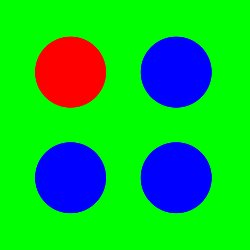
\includegraphics[width=100px]{figures/Marker1}
	\caption{Marker 1 Color}
	\label{fig:markerColor}
\end{figure}

This section focuses on detection of marker 1 (figure \ref{fig:markerColor}) and feature extraction from the given image sequences.
Here very satisfying results have been achieved with both EASY and HARD sequences. To identify the marker a following approach has been used: color segmentation, contour finding and detecting color blobs, filtering all results, getting reference points from the marker. 

\subsection{Segmentation and contours}
For color segmentation method has been implemented. First the image has been converted into HSV color space (figure \ref{fig:c1}), which is better (than RBG) to use with the purposes of computer vision. Then on the HSV image has been applied a threshold (figure \ref{fig:c2}), first using euclidean  distance, which was quite effective for the EASY sequence, but for the HARD sequence an extended threshold range is required (luminosity changes as well as disturbing background). Therefore we used threshold with extended range.

After threshold many small points and small areas remain detected. To eliminate these disturbing features, the morphological 
opening(figure \ref{fig:c3})  is applied first (Erode-Dilate), then closing (figure \ref{fig:c4}) is applied (Dilate-Erode) to fill the small holes. 

To get the contours from the image, findContours() is used. This method records all the found contours on the previously thresholded
image.

\begin{figure}[ht!]
	\begin{subfigure}{.49\textwidth}
		\centering
		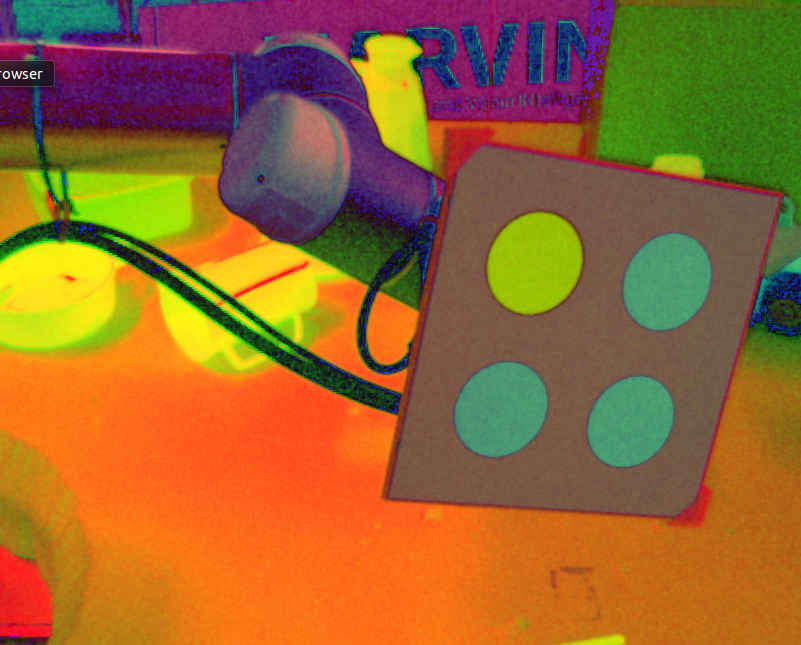
\includegraphics[width=\textwidth]{figures/color1}
	\caption{HSV}
	\label{fig:c1}
	\end{subfigure}
	\begin{subfigure}{\textwidth}
		\centering
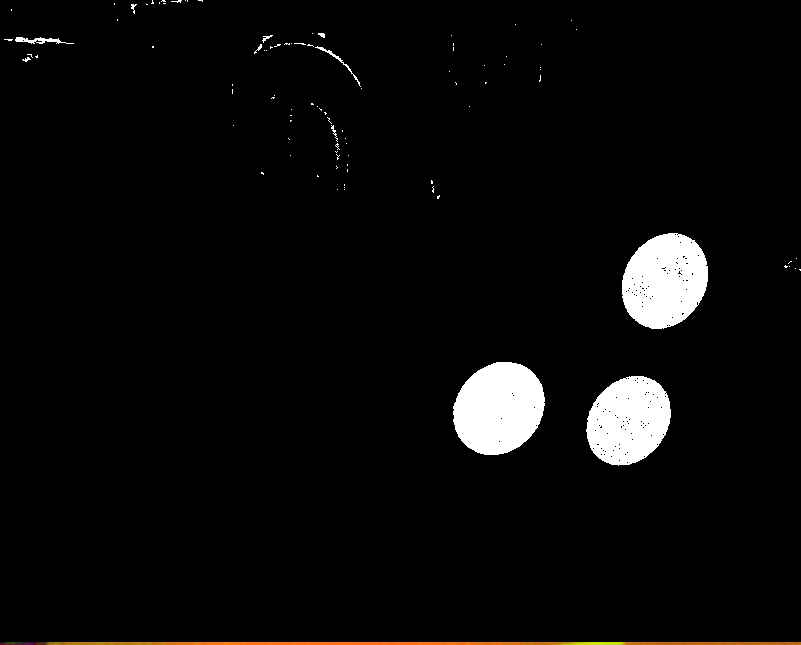
\includegraphics[width=0.5\textwidth]{figures/color2}
	\caption{threshold}
	\label{fig:c2}
	\end{subfigure}
		\begin{subfigure}{.49\textwidth}
		\centering
		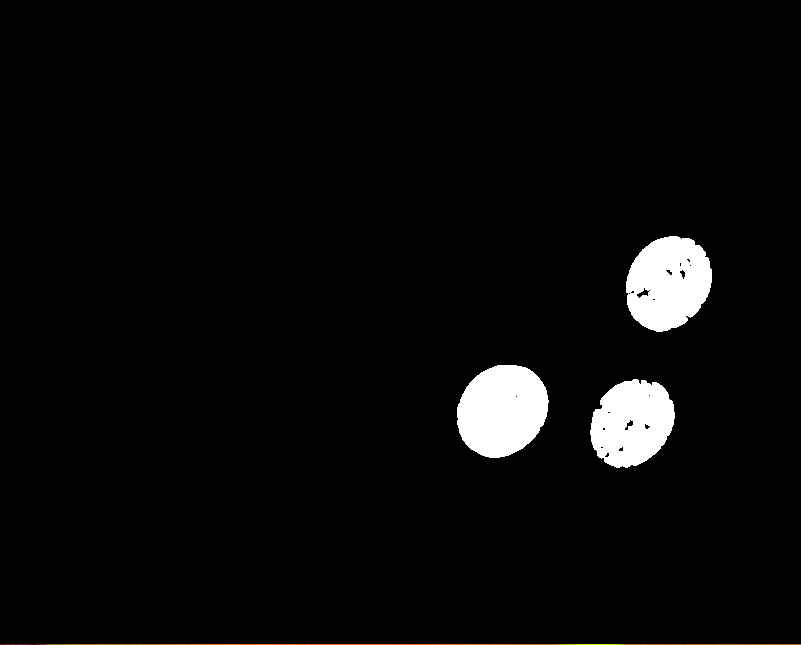
\includegraphics[width=\textwidth]{figures/color3}
	\caption{after morphological Opening}
	\label{fig:c3}
	\end{subfigure}
	\begin{subfigure}{\textwidth}
		\centering
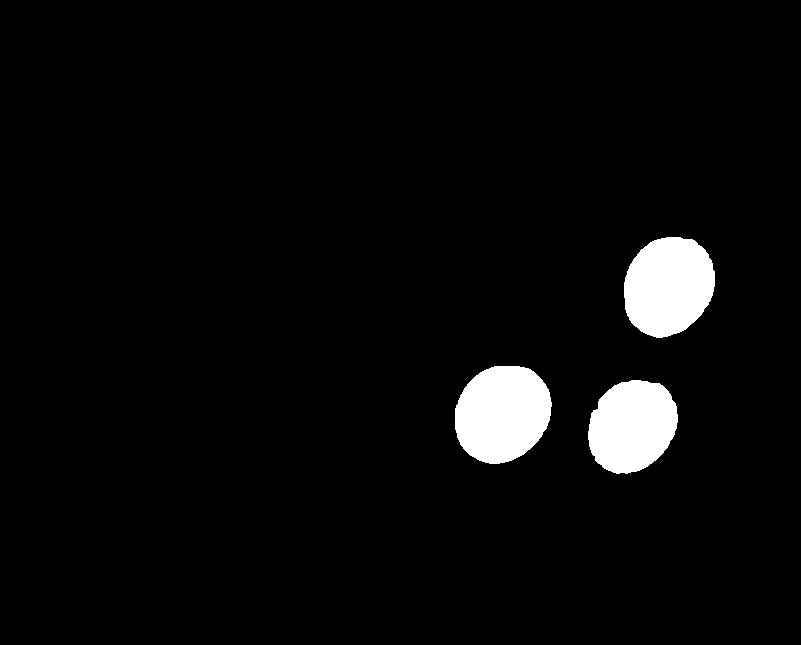
\includegraphics[width=0.5\textwidth]{figures/color4}
	\caption{after morphological Closing}
	\label{fig:c4}
	\end{subfigure}
\caption{HARD sequence - Segmentation}
\label{fig:markerColorSegmenation}
\end{figure}

\subsection{Center of mass}
For calculating the center of mass of the circles several options are available.
One possible solution is to calculate the centre of mass with use of the openCV function
moments() that calculates the moment of a contours and from these moment calculate the
center of mass. This is a very effective solution for calculating the center of mass of
objects with various shapes. This method seems to work perfectly for the easy and quite good
for the HARD sequence. Problem of this method occurs when detecting the marker in the hard sequence,
there sometimes the detected circle contours are not complete (luminosity differences) and the resulting
center of mass is shifted. Of course this problem could be removed by increasing the threshold range, but
then additional contours may occur - this would require improved filtering (by distance, shape) witch would
require more computational time. 



\begin{figure}[ht!]
	\begin{subfigure}{.49\textwidth}
		\centering
		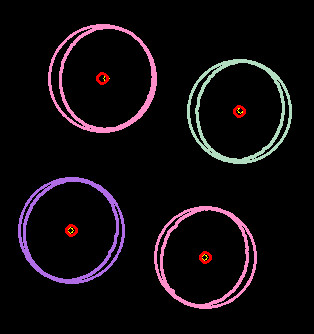
\includegraphics[width=\textwidth]{figures/Marker1centers}
	\caption{Contour view}
	\label{fig:markerColorcenter1}
	\end{subfigure}
	\begin{subfigure}{\textwidth}
		\centering
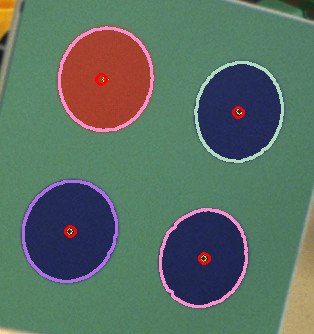
\includegraphics[width=0.5\textwidth]{figures/Marker1centers2}
	\caption{Actual image}
	\label{fig:markerColorcenter2}
	\end{subfigure}
\caption{Center of mass (yellow - moments method, red - minEnclosingCircle)}
\label{fig:markerColorcenter}
\end{figure}

The shapes that need to be detected have circle shapes. For this reason another less time-consuming 
method has been implemented. The center of mass is calculated with function minEnclosingCircle() witch calculates
a surround circle for a given contour. This method also eliminates the marker detection problems with HARD sequence (occurring with
the moments method).When using this function the output circle center point is the center of mass of the detected circle. this method improves the performance over the previously used moment method and the HARD sequence detection then proceeds without problems. This method can be improved with using approxPolyDP() before calling the minEnclosingCircle(). This functions approximates the contour polygon and smoothens possible holes. Without approxPolyDP() the marker detection is faster. 

The difference in outputs of both methods is ranging from 1-5 pixels. When having discovered all the contours very good the first (moments) method is more accurate, but when it comes to problems with damaged contours (luminosity changes) the second method is performing better (figure \ref{fig:markerColorcenter}). 

\subsection{Filtering}

When having extracted all the contours, it is necessary to filter the desired and undesired results. To do so, the bad results are
omitted using the previously calculated contour dimensions (minimal enclosing circle). In the algorithm the position of both, the RED circle and BLUE circles is detected. It is possible both to calculate the center of marker by averaging the points and also export individual points separately. 


\subsection{Marker 1 - Testing and Conclusions}
This feature extraction program was tested with EASY and also HARD sequence. EASY sequence required much less effort (possible to track only the green marker plane). The HARD sequence required much closer analysis. A lot of disturbing features occur there (luminosity changes, background objects with color similarities, etc.). Here the filtering is more important as well as proper
thresholding. The implemented method required advanced tuning and proper parameter settings. 

In the end the marker is detected in all EASY, and also in the HARD sequence. In HARD sequence the detection is very precise when
the marker is facing straight against the camera, when the marker is turned to side (shear), the center of mass detection is around 4 pixels more precise with the moments method (however this method quite fails if the contours are not complete), but otherwise the minEnclosingCircle() method is satisfying. 

The average runtime for HARD is 24.6782 ms, for EASY 17.0602 ms with the complex and precise algorithm. Around 50 ms with the simple algorithm (less precise, one color threshold only - RED, BLUE, or GREEN plate).


\newpage
\section{Marker 2 (2a Thin lines)}

\begin{figure}[ht!]
	\centering
	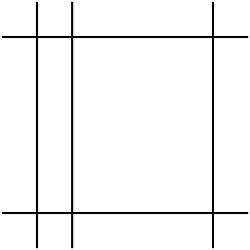
\includegraphics[width=100px]{figures/Marker2a}
	\caption{Marker 2 Thin lines}
	\label{fig:markerLines}
\end{figure}

Detection of lines in the image using the Canny edge detector and the
Hough transform. (Rejection/selection of lines based on the color on
each side). Combining lines to find possible intersections. Verifying
the marker by looking at the distances between intersections. This
approach covers aspect C (and B). This would work with the markers
in Figures 1b and 1c.



\newpage
\section{Marker 3 (Corny)}

\begin{figure}[ht!]
	\centering
	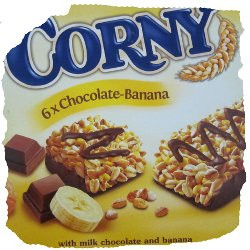
\includegraphics[width=100px]{figures/Marker3}
	\caption{Marker 3 Corny}
	\label{fig:markerColor}
\end{figure}


Extracting SIFT features. Matching the extracted SIFT features against
SIFT features in a marker reference model. Using RANSAC to find
a homography that aligns the reference model with the observations.
Use the homography to transform the marker reference points from
the model to the image. This approach covers aspect D. This would
work with the marker in Figure 1d.
% chapter featre_extraction (end)